%% LaTeX-Beamer template for KIT design
%% by Erik Burger, Christian Hammer
%% title picture by Klaus Krogmann
%%
%% version 2.1
%%
%% mostly compatible to KIT corporate design v2.0
%% http://intranet.kit.edu/gestaltungsrichtlinien.php
%%
%% Problems, bugs and comments to
%% burger@kit.edu

\documentclass[18pt, xcolor=table]{beamer}

%% SLIDE FORMAT

% use 'beamerthemekit' for standard 4:3 ratio
% for widescreen slides (16:9), use 'beamerthemekitwide'
\usepackage[utf8]{inputenc}
\usepackage[T1]{fontenc}
\usepackage{templates/beamerthemekit}
\usepackage{tabularx}
%\usepackage{templates/beamerthemekitwide}

%% TITLE PICTURE

% if a custom picture is to be used on the title page, copy it into the 'logos'
% directory, in the line below, replace 'mypicture' with the 
% filename (without extension) and uncomment the following line
% (picture proportions: 63 : 20 for standard, 169 : 40 for wide
% *.eps format if you use latex+dvips+ps2pdf, 
% *.jpg/*.png/*.pdf if you use pdflatex)

\titleimage{FirstPage}

%% TITLE LOGO

% for a custom logo on the front page, copy your file into the 'logos'
% directory, insert the filename in the line below and uncomment it

\titlelogo{ElipseLogo}

% (*.eps format if you use latex+dvips+ps2pdf,
% *.jpg/*.png/*.pdf if you use pdflatex)

%% TikZ INTEGRATION

% use these packages for PCM symbols and UML classes
\usepackage{templates/tikzkit}
% \usepackage{templates/tikzuml}

% the presentation starts here

\title[Elipse]{Elipse -- Einteilungs Interface für das PSE}
\subtitle{Präsentation Qualitätssicherung}
\author{D. Biester, E. Dohse, P. Faller, P. Loth, L. Seufert, S. Kopmann}
\institute{IPD Snelting}

% Bibliography

\usepackage[citestyle=authoryear,bibstyle=numeric,hyperref,backend=biber]{biblatex}
\addbibresource{templates/example.bib}
\bibhang1em
\beamertemplatenavigationsymbolsempty

\begin{document}

% change the following line to "ngerman" for German style date and logos
\selectlanguage{ngerman}

%title page
\begin{frame}
\titlepage
\end{frame}
\section{Überblick}
\begin{frame}{Überblick}
\begin{itemize}
  \item Vorgehensweise beim Testen
  \item Gefundene und behobene Fehler
  \item Sonstige Verbesserungen
  \item Schwierigkeiten beim Testen
  \item Werkzeug und Statistik
\end{itemize}
\end{frame}

\section{Vorgehensweise}
\begin{frame}{Vorgehensweise beim Testen}
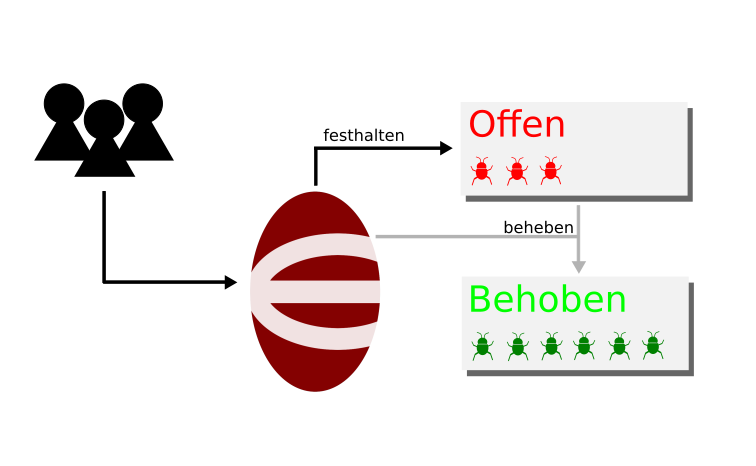
\includegraphics[width=\linewidth]{logos/Vorgehensweise.png}
\end{frame}

\section{Behobene Fehler}
\begin{frame}{Gefundene und behobene Fehler}
\begin{itemize}
  \item EBean Fehler beim:
 	\begin{itemize}
 		\item Beitreten und danach Verlassen einer Lerngruppe
 		\item Erstellen eines Projekts als Betreuer
 		\item erneuten Erstellen eines gelöschten Studenten
 	\end{itemize}
  \item Synchronisation
  	\begin{itemize}
 		\item Betreuer zu Projekt
 		\item SPO/Semester bearbeiten
 		\item Studenten registrieren
 		\item Lerngruppe verlassen, beitreten oder bewerten
 		\item ...
 	\end{itemize}
 	\item Sonstige Fehler
 	\begin{itemize}
 		\item Änderung rückgängig nach Löschen der Einteilung
 		\item Annotation Date-Objekte Datenbank
 		\item Projekt als Betreuer editieren
 		\item ...
 	\end{itemize}
\end{itemize}
\end{frame}

\section{Sonstige Verbesserungen}
\begin{frame}{Sonstige Verbesserungen}
\begin{itemize}
  \item Aktives Semester nur noch außerhalb der Registrierungsphase ändern
  \item Aussagekräftige Fehlermeldungen
  \item GUI verschönert
  \item Speicherverhalten der Tabs im Adminbereich verbessert
\end{itemize}
\begin{figure}
  	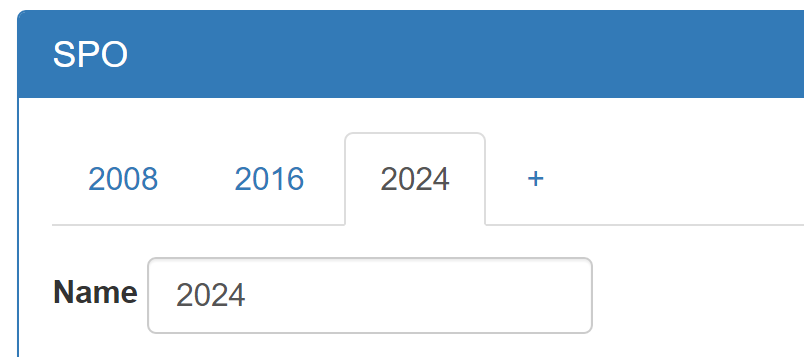
\includegraphics[width=0.5\linewidth]{logos/sonstig1.png}
  \end{figure}
\end{frame}


\section{Schwierigkeiten}
\begin{frame}{Schwierigkeiten beim Testen}
\begin{itemize}
  \item Controller
  \begin{itemize}
  	\item Schwer testbar (mocks)
  	\item Bsp.: Hoch-Herunterladen AdminImportExportController 
  \end{itemize}
  \item Einteilungsberechnung
  \begin{itemize}
  	\item Kriterien sind notwendig aber nicht hinreichend für die Funktion	
  \end{itemize}
  \item EBean, Löschen aus der Testdatenbank
\end{itemize}
\end{frame}

\section{Werkzeug und Statistik}
\begin{frame}{Werkzeug und Statistik}
	SonarQube:
	\begin{figure}
  			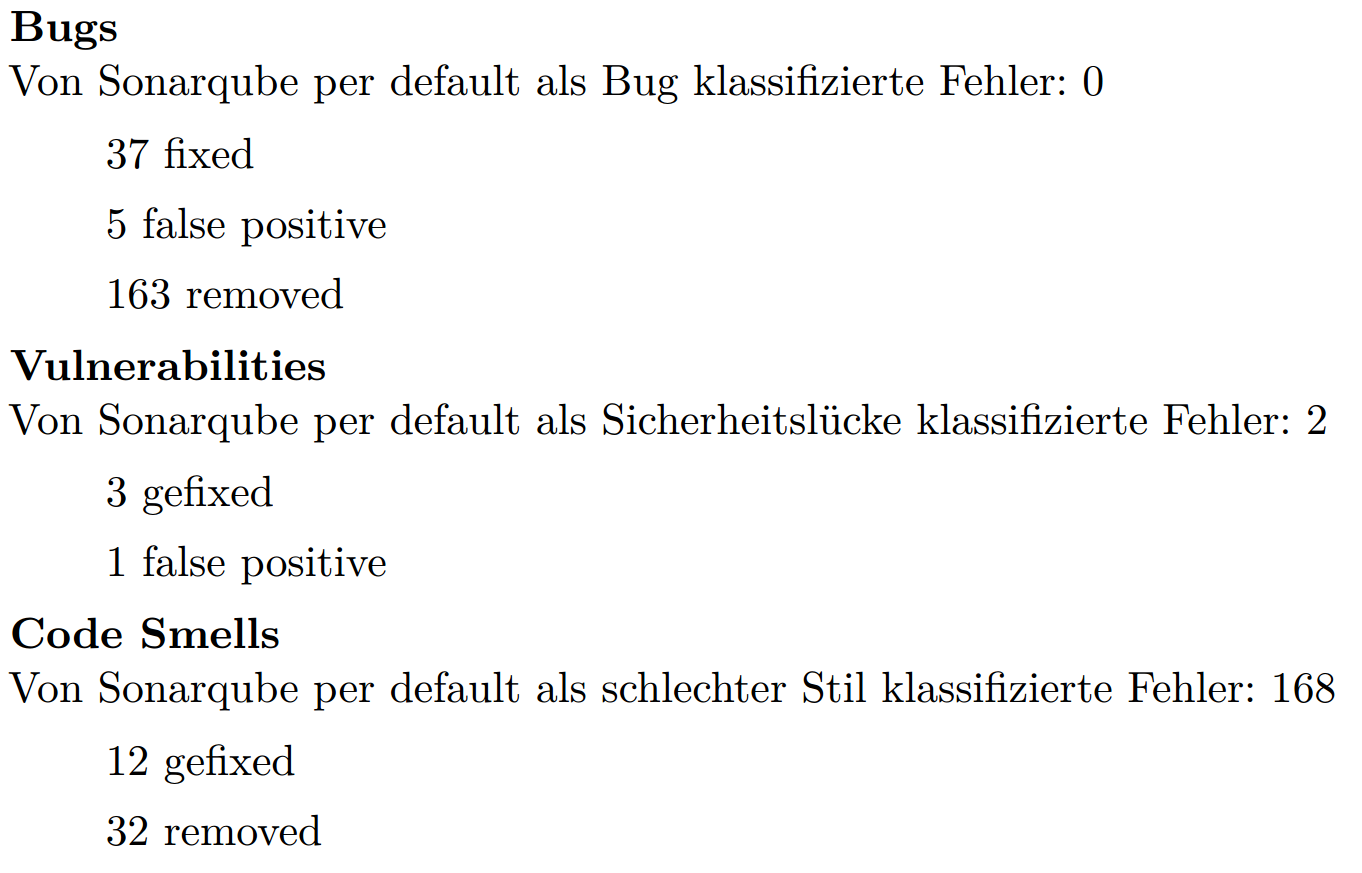
\includegraphics[width=0.7\linewidth]{logos/SonarQubeStat.png}
  		\end{figure}
\end{frame}

\begin{frame}{Statistik}
	Java Code Coverage:
	\begin{figure}
  			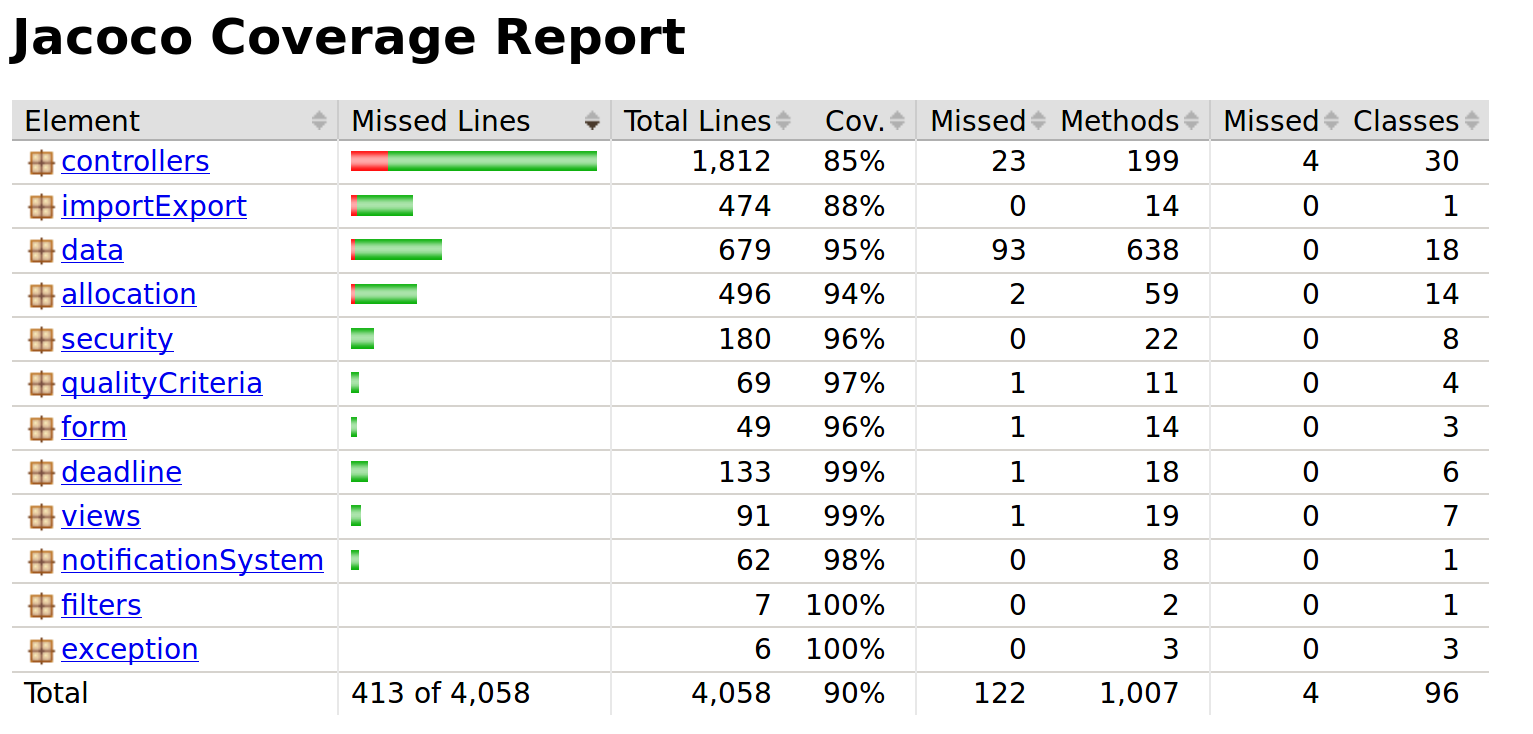
\includegraphics[width=0.85\linewidth]{logos/jacoco.png}
  		\end{figure}
\end{frame}

\begin{frame}{Statistik}
	Lines of Code:
	\begin{figure}
  			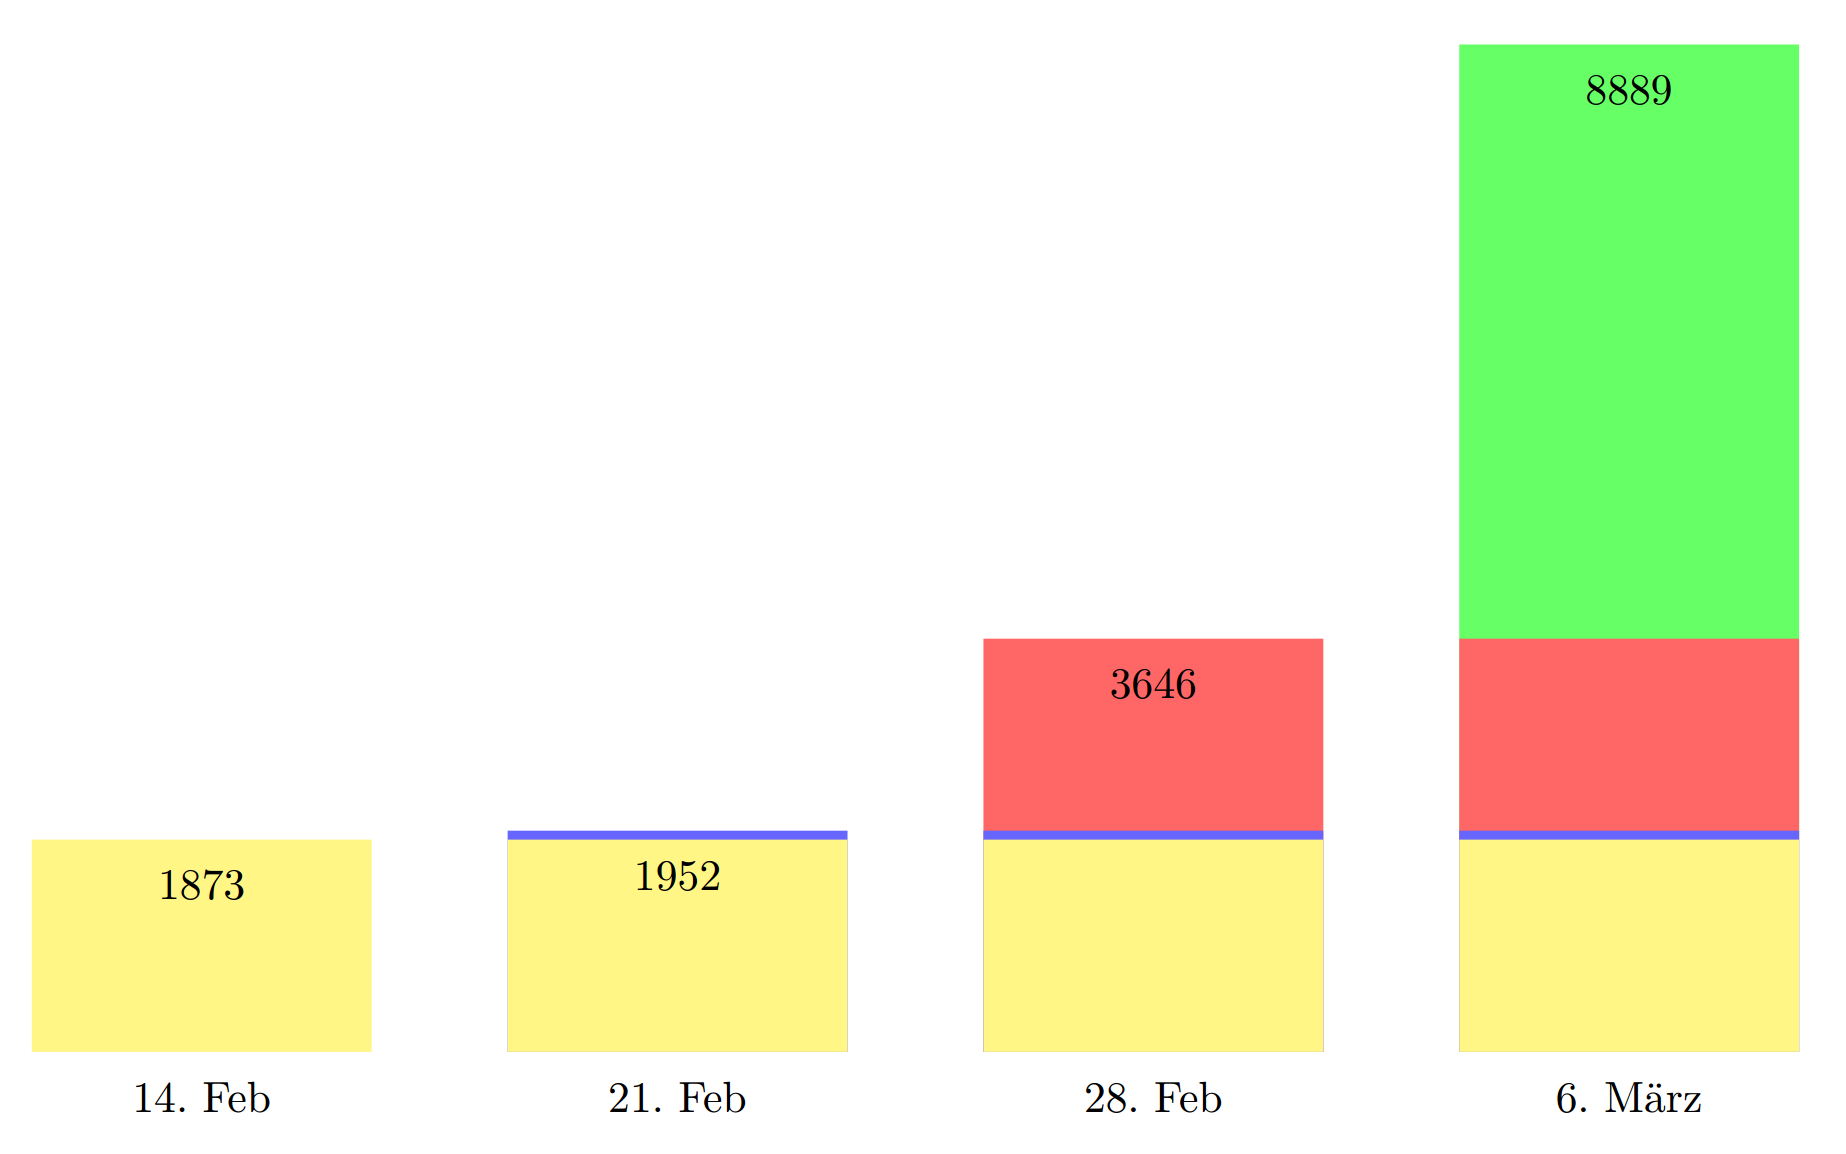
\includegraphics[width=0.8\linewidth]{logos/linesOfCode.png}
  	\end{figure}
\end{frame}

\appendix
\beginbackup

\begin{frame}{Fragen}
\printbibliography
\end{frame}

\backupend

\end{document}
